\section{Directed and Undirected Graphs}
\annote{refference ti l figuren virker ikke}
Figure \cref{labeled_Directed_undirected} shows two graphs, one which is directed and another one which is undirected. Graph 1 is undirected and don't have a specific direction. Graph 2 is directed which means the edges is one way only. The arrows indicates the direction the edges allow. This means vertex 1 can go to vertex 2 and 3, but neither can go back. 


\begin{figure}[ht!]
    \centering
    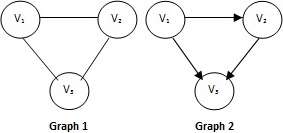
\includegraphics[width=0.5\textwidth]{Directed_undirected.png}
    \label{fig:labeled_Directed_undirected}
    \caption{Graph 1 is directed were graph 2 is undirected \newline Picture from Differencebetween.com\cite{dir_pic}}
  \end{figure}